\Hefteintrag{1}{SQL Spickzettel}{
    \AttachVlg{\faFilePdfO}{_Hefteintraege/img/SQL-Spickzettel_2on1.pdf}

    \ifbeamer\else\vspace{12pt}\fi
    Folgender SQL-Spickzettel enthält alle SQL-Grundlagen der 9. Klasse. Ihr dürft (sollt!) ihn bei allen SQL-Aufgaben benutzen. Über das Vorlagensymbol~~~\faFilePdfO~~~ oben könnt ihr den Spickzettel als eigenes PDF öffnen.
    
    \hinweis{Übrigens: \emphColA{SQL} ist die Abkürzung für \emphColA{S}tructured \emphColA{Q}uery \emphColA{L}anguage, was auf Deutsch etwa Strukturierte Abfrage Sprache heißt.}
    \begin{tcolorbox}[
        boxrule=0pt,        % Kein Rand um die Box
        enhanced,           % Erweiterte Optionen aktivieren
        colback=white,      % Hintergrundfarbe der Box auf Weiß setzen
        frame hidden,       % Rahmen ausblenden
        boxsep=-10mm
    ]
        \centering
        \ifbeamer
            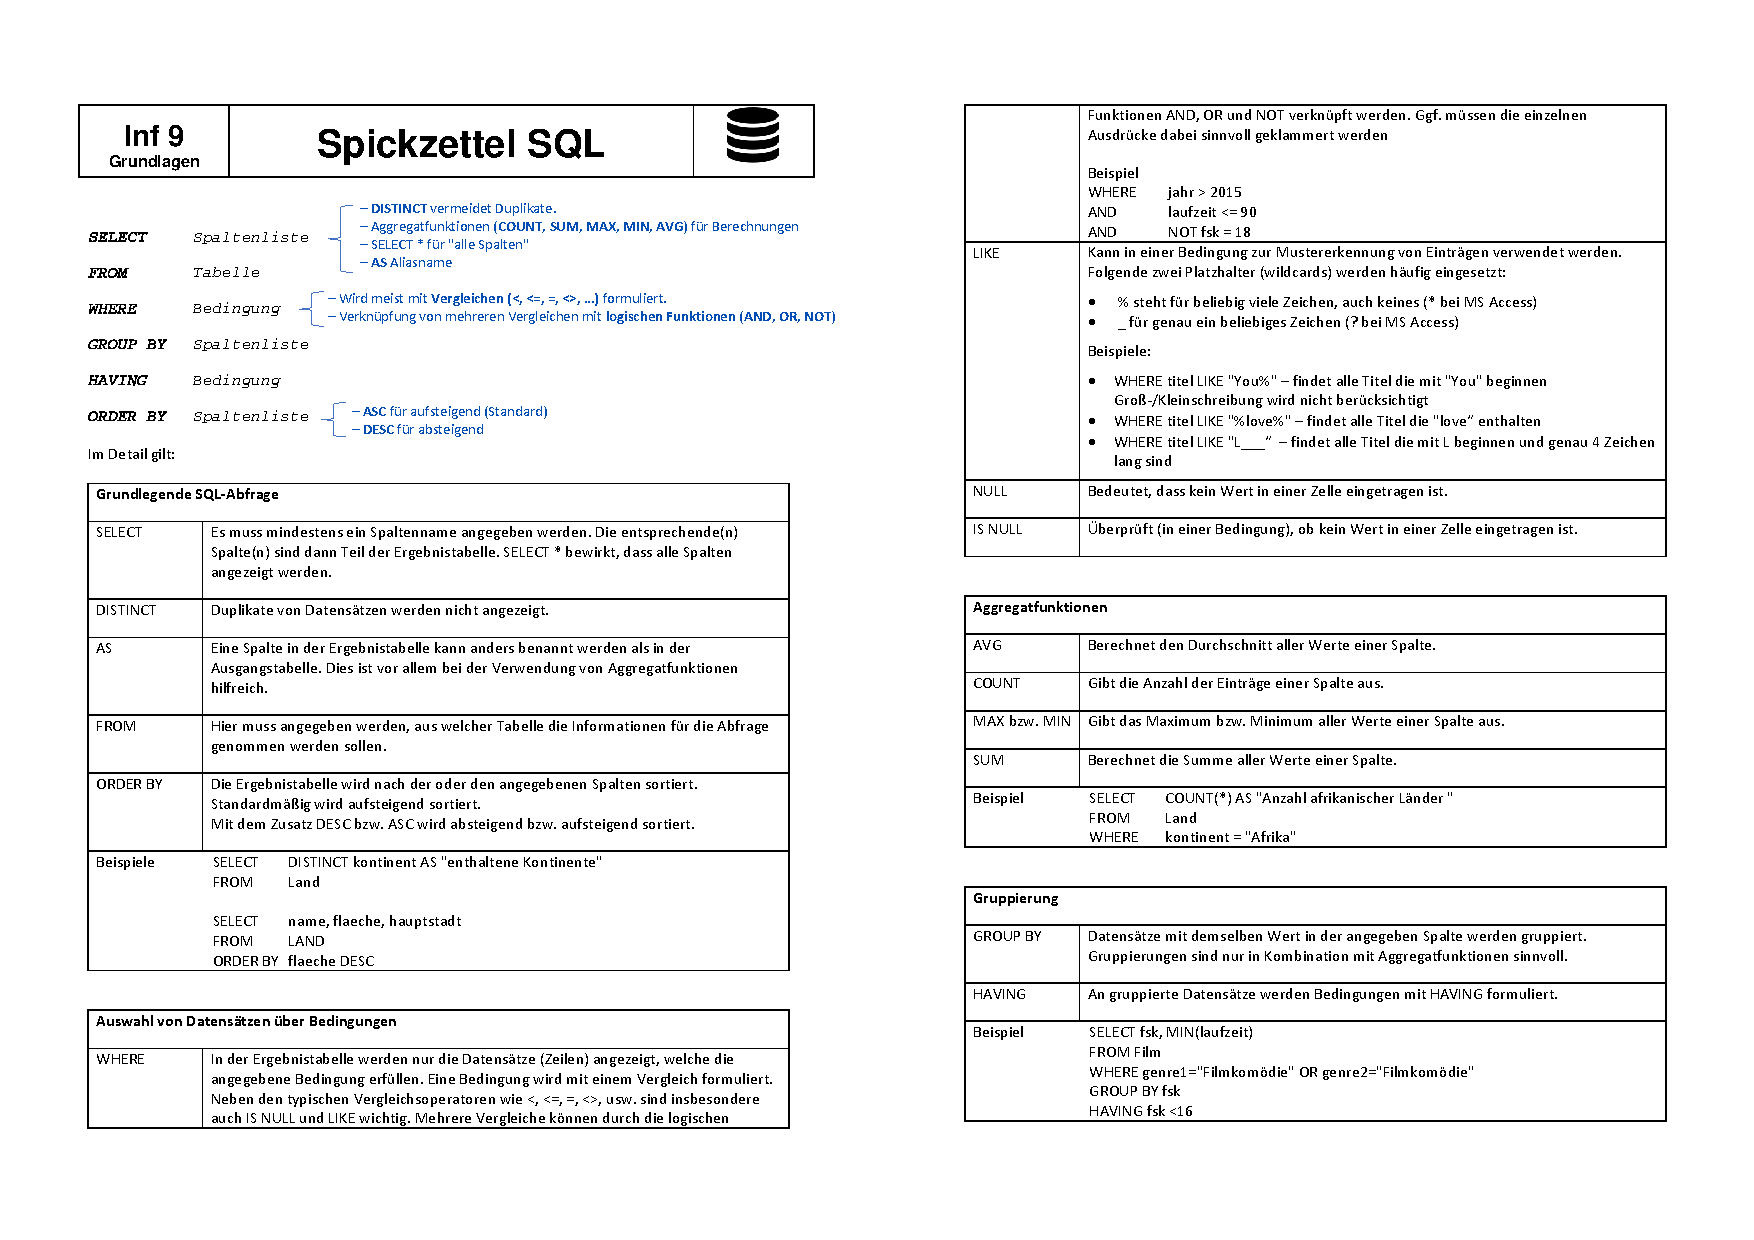
\includegraphics[width=0.68\textwidth]{_Hefteintraege/img/SQL-Spickzettel_2on1.pdf}
        \else
            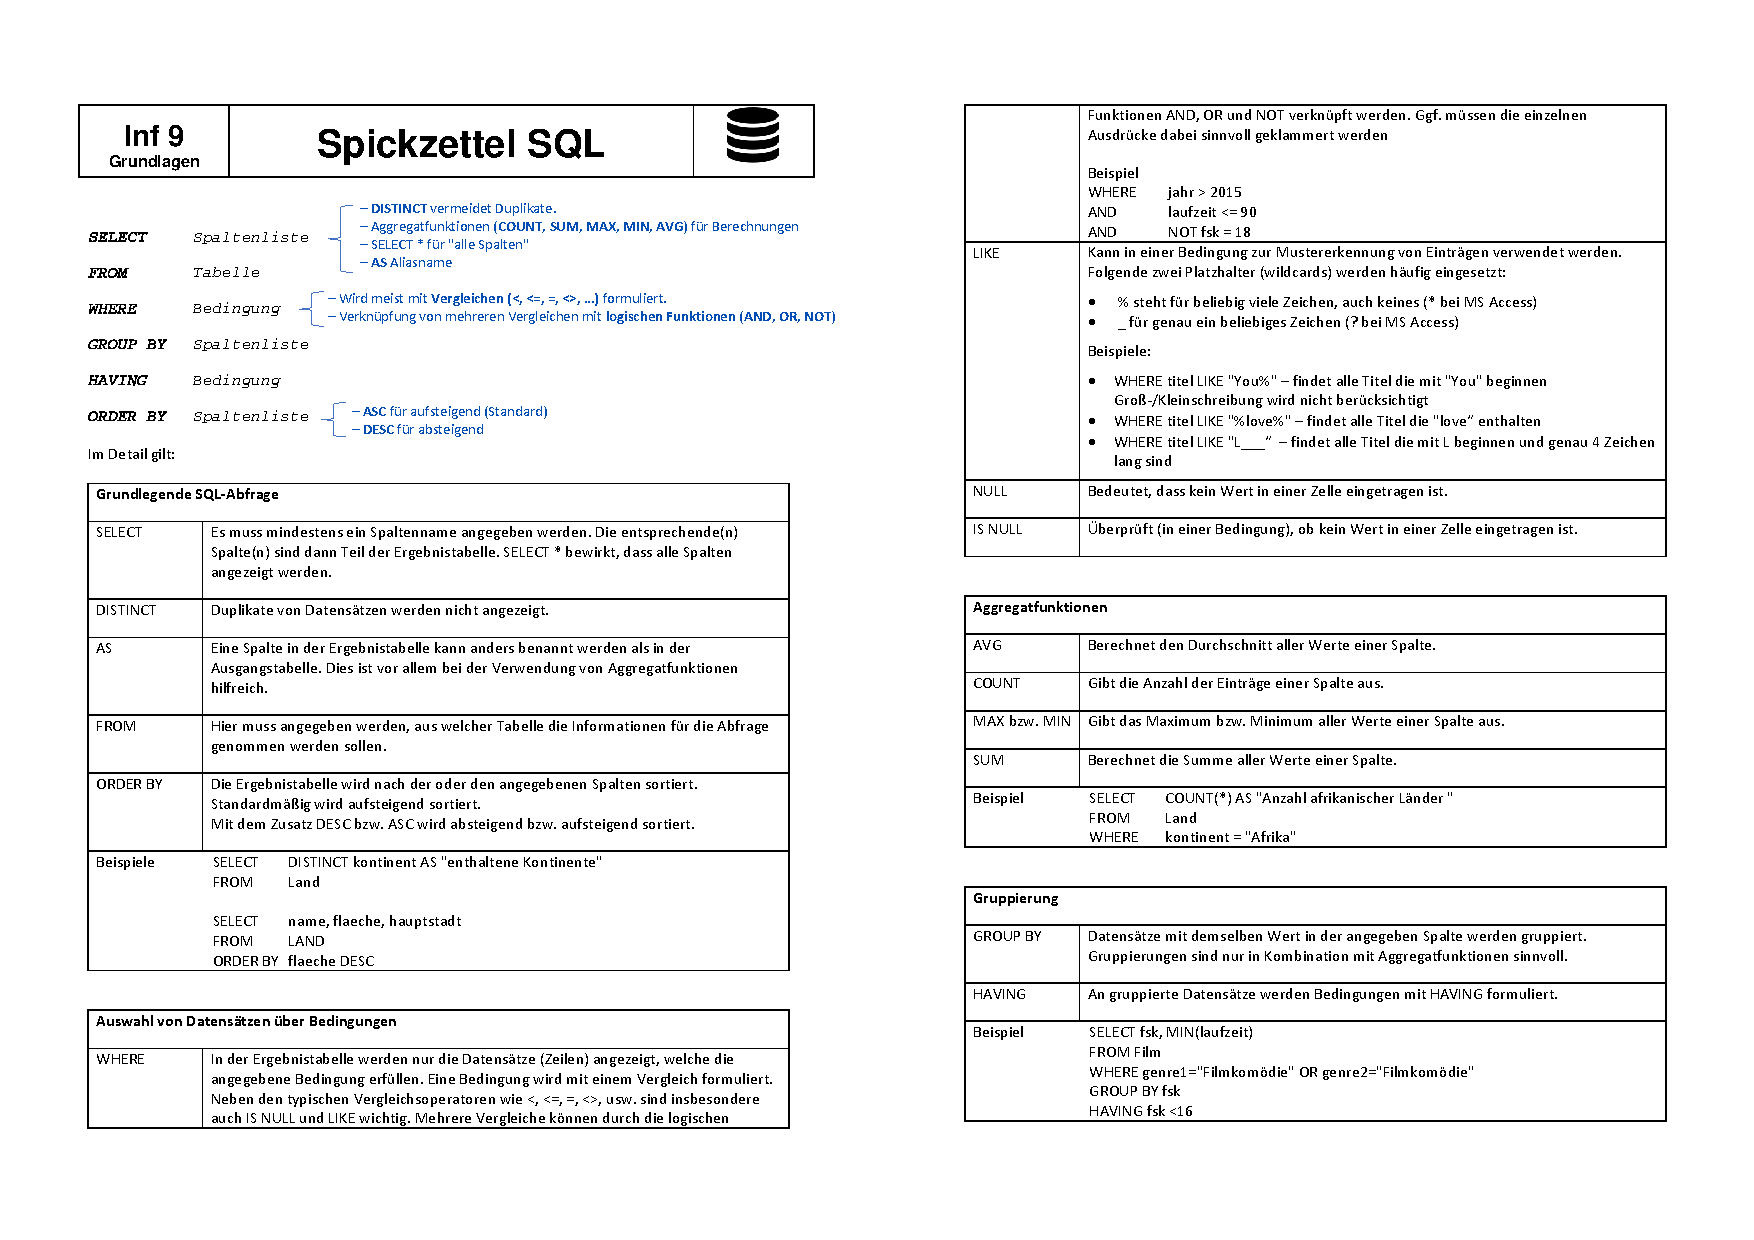
\includegraphics[width=\textwidth]{_Hefteintraege/img/SQL-Spickzettel_2on1.pdf}
        \fi
    \end{tcolorbox}
}
\newcommand{\sqlmemes}{
    \doppelseite{0.43}{0.5}{c}{
        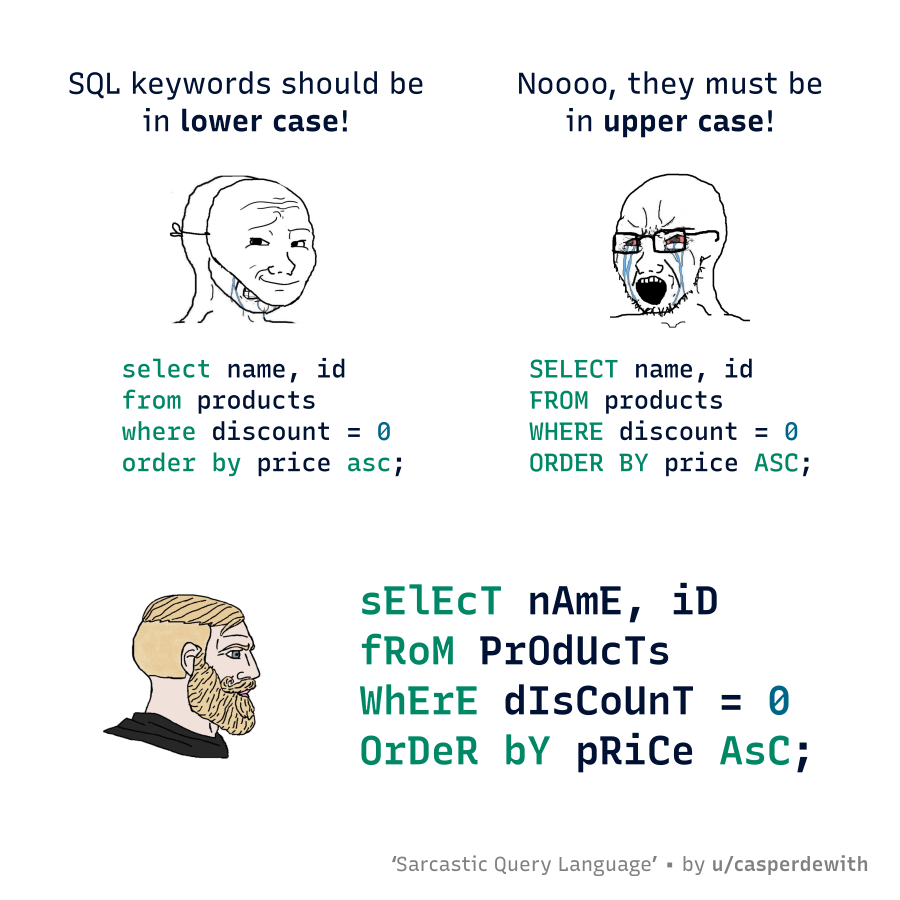
\includegraphics[width=\textwidth]{_Hefteintraege/img/sql_meme_1.png}
        
        \hinweis{SQL Schlüsselwörter wie SELECT, WHERE etc. sind nicht case-sensitive. Groß-/Kleinschreibung ist also egal.}
    }{
        
\includegraphics[width=\textwidth]{_Hefteintraege/img/sql_meme_2.png}
    }
}
\ifbeamer
\definesframe[false]{SQL Memes}{\sqlmemes}
\else
\sqlmemes
\fi